\documentclass[UTF8,fontset=windows,a4paper,10.5pt]{ctexart}
\usepackage[margin=2.05cm]{geometry}
\usepackage{amsmath,amssymb,bm,booktabs,tabularx,array,graphicx,float,xcolor}
\usepackage{caption,enumitem,fancyhdr,hyperref,microtype,lastpage}
\definecolor{blue}{HTML}{0072B2}\definecolor{green}{HTML}{009E73}\definecolor{orange}{HTML}{D55E00}
\hypersetup{colorlinks=true,linkcolor=blue,urlcolor=blue,citecolor=green,pdftitle={SAR ADC校准算法Python验证与硬件代价报告}}
\graphicspath{{../results/figures/}}
\captionsetup{font=small,labelfont=bf}
\setlist{itemsep=0.15em,topsep=0.25em}
\renewcommand{\arraystretch}{1.15}
\pagestyle{fancy}\fancyhf{}\fancyhead[L]{CODEX\_VERI v0.3.0}\fancyhead[R]{Python阶段结论}\fancyfoot[C]{\thepage/\pageref{LastPage}}\setlength{\headheight}{14pt}
\newcommand{\pass}{\textcolor{green}{\textbf{通过}}}
\newcommand{\fail}{\textcolor{red!75!black}{\textbf{未通过}}}
\newcommand{\warn}{\textcolor{orange}{\textbf{有条件}}}

\begin{document}
\begin{titlepage}\centering
\vspace*{2.0cm}
{\Huge\bfseries SAR ADC递归权重校准算法\par}\vspace{0.4cm}
{\LARGE\bfseries Python完整验证、硬件代价与方案决策报告\par}\vspace{1.2cm}
{\large 12位、14次判决冗余CDAC；目标 ENOB $>11.5$ bit\par}\vspace{1.5cm}
\begin{tabular}{rl}
工程：& \texttt{CODEX\_VERI}\\
版本：& \texttt{0.3.0-python-enob-q2}\\
主随机种子：& \texttt{2026072202}\\
物理Monte Carlo：& 2000组（两个相干频点，共4000条）\\
报告日期：& 2026年7月22日\\
生成：& XeLaTeX\\
\end{tabular}
\vfill
\fbox{\parbox{0.89\textwidth}{\small\textbf{最终审查结论：整体FAIL，动态条件通过。}候选重构在明确的Python物理失配模型下达到动态ENOB门槛；但内部校准权重仍为浮点，尚未闭合Q6权重、有限位宽累加与归一化舍入，且Q2静态曲线仍见小回退。因此本报告不授权进入VA，也不能写成完整INL/DNL或硬件实现通过。}}
\vfill
\end{titlepage}
\tableofcontents\clearpage

\section{执行结论}
\begin{enumerate}
\item 已复现并定位历史约$0.3\%$的逐级权重漂移。根因不是Huang方法要求每级乘固定修正，而是旧实现把非负幅度量化误差递归注入后续级。采用\textbf{带符号中心残差（wall+signed）}并令trial exact tie立即结束后，理想七级误差为零，奇对称性误差为零。
\item 当前12-bit整数输出即使增加到128对平均也\fail：仅19/4000通过，最差ENOB 11.0634 bit。主要瓶颈是物理SAR量化后，校准权重产生小数码，再舍入至12-bit引入第二次约$1/\sqrt{12}$ LSB量化噪声。
\item 最低数字代价可行点为\textbf{Q2固定点重构（保留2个小数位）+128对校准}：4000/4000通过，最差11.5213 bit，1\%分位11.5611 bit，单侧95\%良率下界99.925\%。
\item Q2不改CDAC、不增加正常转换比较周期；代价是输出由12 bit扩展为14-bit fixed-point，重构数据通路和累加器增加位宽。128对使前台校准由67.2~$\mu$s增至268.8~$\mu$s。
\item 王巍等2022年的自测量方法值得作为\textbf{缩短前台测量时间的候选}，但其最终仍依赖$D_{CAL}=\sum D_iW_i$的加权输出，论文未交代权重小数位和最终接口舍入，故它\textbf{不能直接解决本项目已观察到的12-bit二次量化瓶颈}。
\item Q2最差静态样本存在$-0.25$至$-0.5$ LSB小回退；因此Python动态阶段通过，但进入VA后必须同时检查码密度DNL/INL与单调性。
\item 独立审查结论为\fail（整体）：当前程序的校准权重仍以浮点保存，Q2只约束最终输出。必须补做内部Q6权重、真实累加器位宽、归一化和逐级舍入后，才可称硬件闭环完成。
\end{enumerate}

\section{被验证的系统与计数}
物理判决权重为
\[
\bm W=[2080,1040,520,260,130,65_R,65_A,64,32,16,8,4,2,1].
\]
正常信号权重取索引$[0,1,2,3,4,6]$，名义和为4095；辅助/冗余权重和为192；全部权重和4287。物理SAR判决与数字译码在程序中完全分离，译码采用
\[
D=\mathrm{clip}\!\left(\mathrm{round}\left[4095\frac{S-W_{aux}/2}{W_{sig}}\right],0,4095\right).
\]
校准共有7级、每级正负两个方向。32对时为$7\times32\times2=448$个RST1 frame，而不是4480个frame；4480是CAL\_CLK判决总数。150 ns/frame下理论时间67.2~$\mu$s。128对为1792 frame、268.8~$\mu$s。

\section{校准数学修复与反证}
旧递归把幅度域误差直接加到上一层wall，非负量化偏差会逐级放大。候选改为
\[
\widehat W_k=W_{wall,k}+Q_s(W_k-W_{wall,k}),\qquad Q_s(-x)=-Q_s(x),
\]
并区分两类tie：trial阶段精确命中时接受trial并直接结束，terminal tie只作用于真正到达terminal的路径。这样避免H1C-R在精确65 LSB后又追加1 LSB。

35项单元测试全部通过，覆盖：trial/terminal tie分离、奇对称、饱和显式失败、D+/D-日志一致性、7级$\times$32对覆盖、噪声$1/\sqrt N$律、连续灵敏度矩阵、相干FFT与时域最小二乘交叉检查。

\begin{figure}[H]\centering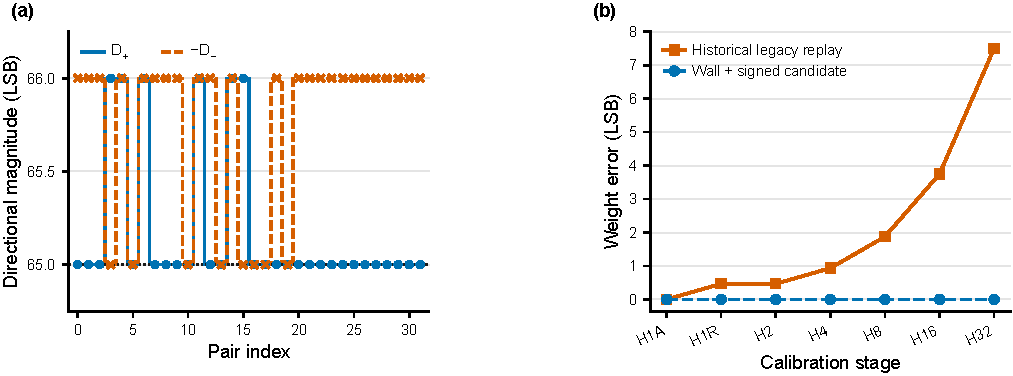
\includegraphics[width=.93\linewidth]{fig01_legacy_bias_replay.pdf}\caption{历史递归偏差重放与带符号中心残差修复。}\end{figure}

\section{动态性能正式门禁}
测试采用8192点、矩形窗、互素相干频点127和3641、输入$-0.915$ dBFS。SNDR包含除直流和基波外的全部频谱能量，不删除谐波；每条记录同时用FFT和时域正弦最小二乘交叉核对。硬门槛为未四舍五入的
\[
\mathrm{ENOB}>11.5\quad\Longleftrightarrow\quad \mathrm{SINAD}>70.99\ \mathrm{dB}.
\]
单位电容失配$\sigma=1\%$（截断于$3\sigma$），校准噪声0.75 LSB、校准offset标准差0.5 LSB、正常转换噪声0.15 LSB。

\begin{table}[H]\centering\small
\caption{正式4000条动态记录结果。}
\begin{tabular}{lrrrrl}\toprule
方案&通过数&最差ENOB&1\%分位&中位数&判定\\\midrule
名义权重，12-bit&0&8.2509&8.7626&9.8472&\fail\\
32对校准，12-bit&9&10.8906&11.0771&11.2188&\fail\\
128对校准，12-bit&19&11.0634&11.1526&11.2467&\fail\\
128对校准，Q2&4000&11.5213&11.5611&11.6137&\pass\\
3个sub-LSB判决，12-bit&4000&11.5597&11.5893&11.6429&\pass（高模拟代价）\\
理想分数抵消oracle，12-bit&4000&11.5865&11.6100&11.6546&仅上界\\\bottomrule
\end{tabular}
\end{table}

\begin{figure}[H]\centering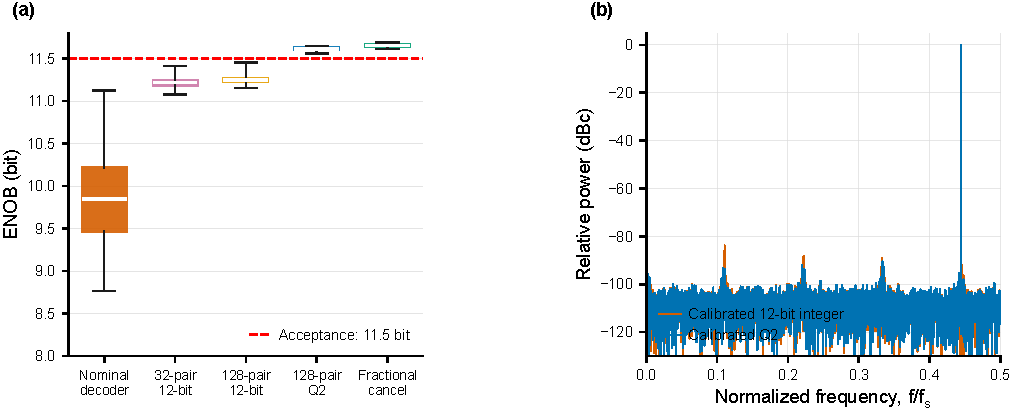
\includegraphics[width=.95\linewidth]{fig06_adc_enob_and_spectrum.pdf}\caption{ENOB分布与最差样本频谱；红虚线为11.5-bit门槛。}\end{figure}

\subsection{为何12-bit整数路径失败}
失配校准后，$\sum D_iW_i$通常不是整数。若末端再次舍入，理想SAR量化噪声和重构舍入噪声近似独立：
\[
\sigma_q\simeq\sqrt{\frac1{12}+\frac1{12}}=0.4082\ \mathrm{LSB},
\]
相对单次量化恶化约3.01 dB，即约0.5 bit。这解释了“权重估计很准但ENOB仍停在约11.2--11.4 bit”的现象。增加平均次数只降低权重估计噪声，不能消除正常转换中的第二次量化。

\section{静态结果与硬件代价}
Q2候选对挑选的最差动态样本做262144点静态斜坡。端点拟合峰值误差均小于0.93 LSB，但三个样本分别出现1、25、8次回退，最坏回退$-0.5$ LSB。因此动态门禁\pass，而完整静态签核\warn。

\begin{figure}[H]\centering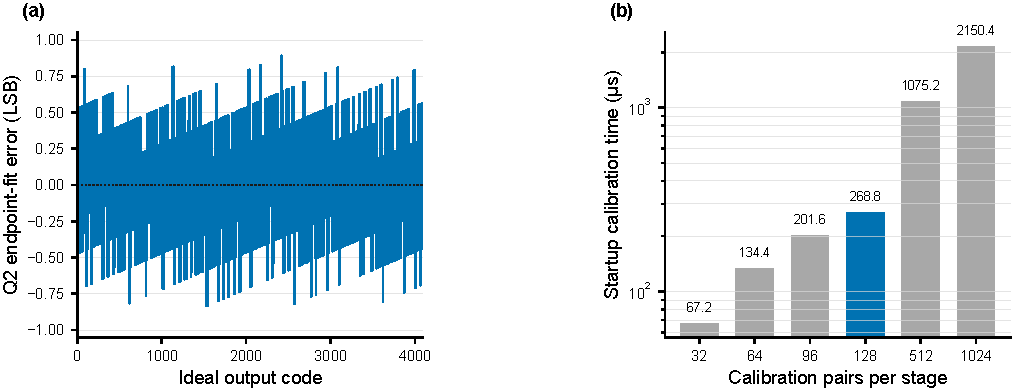
\includegraphics[width=.95\linewidth]{fig07_static_and_hardware_cost.pdf}\caption{Q2静态端点拟合误差与前台校准时间。}\end{figure}

\begin{table}[H]\centering\small
\caption{候选方案的硬件/时间Pareto比较。}
\begin{tabularx}{\textwidth}{p{2.2cm}p{3.2cm}Xp{2.4cm}}\toprule
方案&模拟/时序代价&数字接口代价&判断\\\midrule
32对12-bit&无新增；67.2~$\mu$s&现有12 bit&ENOB不通过\\
128对Q2&无新增；正常周期+0；268.8~$\mu$s&输出+2 bit；累加器约19--20 bit&\textbf{首选}\\
Q6数字输出&无新增；268.8~$\mu$s&输出+6 bit，带宽+50\%&过度设计\\
512/1024对&无新增；1.075/2.150 ms&计数器增宽&时间高且不治二次量化\\
3个sub-LSB判决&分数CDAC/开关；至少+3周期&保持12 bit&性能好，模拟风险高\\
上下文LUT&无模拟新增&可能为多Mbit存储&面积过高，拒绝\\\bottomrule
\end{tabularx}
\end{table}

Q2的关键现实条件是：\textbf{下游必须接收14-bit fixed-point，或在数字域继续以Q2计算。}若芯片引脚/协议只能输出12 bit并立即舍入，Q2收益将被重新量化抹掉，此时只能另行设计噪声整形/过采样输出，或承担模拟分数抵消的代价。

\section{对王巍等2022方法的独立评价}
论文以$011\ldots1\leftrightarrow100\ldots0$切换产生位电容误差，分别测量P/N两侧：
\[
\Delta V_p=-V_{ep}+V_{os},\quad \Delta V_n=V_{en}+V_{os},\quad
V_e=-\Delta V_p+\Delta V_n.
\]
它的优点是复用主CDAC、比较器和LSB段逐次逼近，不需要LMS或矩阵求逆；论文报告约15个采样周期，因而很适合研究为本项目现有448-frame流程的\textbf{快速测量前端}。

但迁移前有五个硬条件：
\begin{enumerate}
\item 必须满足sub-radix/冗余覆盖，否则偏大的位电容导致模拟信息丢失，数字校准无法恢复。本项目冗余覆盖有利，但需逐级做最坏角证明。
\item 静态offset只在两次测量之间近似不变时才能抵消；动态offset、噪声、切换注入、P/N路径不对称仍会残留。
\item LSB段被当成测量ADC，其自身失配、桥接寄生和建立误差决定测量下限，论文未给出面向本项目1\%单元失配的尾部良率。
\item 实现仍需P/N独立切换、直流/VCM采样状态、控制FSM、权重寄存器和每次转换的加权求和，不能按“零硬件”估算。
\item 最重要的是论文式(9)仍为分数权重加权输出，未说明定点小数位和最终码宽；其15.38-bit仿真不能证明压回16-bit整数后仍保持同一ENOB，也不能直接治愈本项目12-bit二次量化。
\end{enumerate}
因此本轮不把它替换为主方案。建议后续Python分支仅验证其\textbf{测量速度/估计方差}，译码仍先采用已通过的Q2基线；若VA中证实15-cycle测量可靠，再用它降低268.8~$\mu$s启动时间。

\section{阶段决策与VA入口条件}
\textbf{Python动态ENOB：通过；Python整体硬件闭环：未通过。}最低硬件代价候选为“wall+signed、trial exact stop、128对、Q2输出”，但尚未冻结为VA基线。现有12-bit整数接口明确不通过，且浮点权重必须替换为内部Q6定点实现后重新跑4000条门禁。

进入VA之前的剩余入口检查为：
\begin{enumerate}
\item 保持RST1=150 ns、CAL\_CLK=10 ns，不以压缩建立时间加速；
\item 导出D+、D-、signed residual、accepted sum、terminal状态和实际DONE时间；
\item Python先实现内部Q6权重、约20-bit累加器和可综合归一化/舍入；通过后VA内部保留Q2输出，并对照末端12-bit舍入；
\item 先1对做tie/极性定向，再128对做完整动态回归；
\item 同时做码密度DNL/INL，任何$-0.5$ LSB回退必须解释或修复后方可签核。
\end{enumerate}

\section{可复现性与参考资料}
一键门禁：\texttt{powershell -ExecutionPolicy Bypass -File .\\run\_python\_gate.ps1}。原始汇总为\texttt{results/raw/adc\_performance\_summary.json}；4000条记录、静态斜坡和硬件时间表位于\texttt{results/tables/}。全部写入仅发生在\texttt{CODEX\_VERI/}。

\begin{thebibliography}{9}\small
\bibitem{ieee1241} IEEE Std 1241-2023, \emph{Terminology and Test Methods for Analog-to-Digital Converters}.
\bibitem{ti} Texas Instruments, \emph{Coherent Sampling vs. Window Sampling}, SLVAG04.
\bibitem{huang} S. Huang, \emph{Advanced Clock Multiplier and SAR ADC Design Techniques for High-Resolution Signal Chain Systems}, Ph.D. dissertation, 2024.
\bibitem{wang2022} 王巍等，“一种SAR ADC电容失配自测量与数字校准技术”，《微电子学》，52(4), 550--554, 2022, DOI: 10.13911/j.cnki.1004-3365.210333.
\bibitem{zhang2019} Zhang et al., “A 16-bit 1-MS/s Pseudo-Differential SAR ADC With Digital Calibration,” \emph{IEEE Access}, 2019, DOI: 10.1109/ACCESS.2019.2937384.
\end{thebibliography}

\end{document}
